\documentclass[10pt, conference, compsocconf]{IEEEtran}
\IEEEoverridecommandlockouts
\usepackage{graphicx}
\usepackage{color}
\usepackage{balance}
\usepackage{multirow}
\usepackage{listings}
\newtheorem{property}{Property}
\lstset{breaklines=true, basicstyle=\scriptsize, %frame=single, 
  keywordstyle=\color{blue}, commentstyle=\color{green},
  identifierstyle=\color{cyan},
  stringstyle=\ttfamily\color{red}, showstringspaces=false,
  language=Java, numberfirstline=true,
%  frameround=false, frame=trBL
}
\title{Specifying and Detecting Relevant Changes\\ in Programs}
\author{\IEEEauthorblockN{
Yijun Yu\IEEEauthorrefmark{1},
Thein Than Tun\IEEEauthorrefmark{1} and
Bashar Nuseibeh\IEEEauthorrefmark{1} \IEEEauthorrefmark{2}}
\IEEEauthorblockA{\IEEEauthorrefmark{1}
The Open University\\
Milton Keynes, UK\\
Email: \{t.t.tun, y.yu, b.nuseibeh\}@open.ac.uk}
\IEEEauthorblockA{\IEEEauthorrefmark{2}
Lero,  Irish Software Engineering Research Centre\\
Limerick, Ireland\\
Email: bashar.nuseibeh@lero.ie}}
\newtheorem{definition}{Definition}
\begin{document}
\maketitle
\begin{abstract}
Software developers are primarily interested in the changes in code that are
relevant to their current tasks, therefore not all changes to evolving software
are of the same importance. However, most existing {\tt diff} tools notify
developers more changes than they wish to see.  In this paper, we propose an
automated technique to specify and detect only those relevant changes in
programs in order to avoid looking at other trivial changes.  Using four
elementary extensions to programming language grammars (Ignore, Order, Prefer and
Keep), developers can specify, with limited effort, what types of changes are
relevant to their programming tasks. The algorithms for generating the
normalisation and clone removal transformations distill the non-trivial or
meaningful differences automatically.  Our tool has been evaluated on a
benchmark of programs to demonstrate its improved precision comparing with
other {\tt diff} techniques.  
\end{abstract}
\section{Introduction}

``Nothing endures but change.'' -- Heraclitus (c.535 BC - 475 BC). This philosophy is largely true in most software development projects. However, not all changes are equally meaningful to different purposes. For example, changing the indentations of statements does not necessarily alter the meanings or semantics expressed by a program. Nonetheless it could lead to false alarms to any revision control system as text-based difference comparison algorithms are typically used (e.g., the {\bf diff} utility in Unix~\cite{diff}). Although an indentation is not meaningful to the executation semantics of C/Java programs, it can be very important to other programming languages such as Python. Still can it be meaningful to C/Java developers who care about pretty-prints for the sake of code reviews. Another example is the API evolution: thanks to the widely adopted information hiding and modular design principle~\cite{Parnas:1972:CUD:361598.361623}, users of object-oriented programming libraries are encouraged to neglect any changes behind the API. Therefore detecting changes to the API of software components becomes meaningful~\cite{DBLP:journals/smr/DigJ06}. On the other hand, providers of the API need to pay attention to most changes inside the API implementation. 

Given that a change considered as meaningful for one purpose may be trivial to another, how can one specify the types of changes to be detected for this given purpose? Furthermore, how can such a specification be used for an automatic detection? Most change detection tools are either good at reporting {\em all} changes through general purpose diff algorithms on programs represented as line-separated text~\cite{diff, canfora09software} and structured models~\cite{DBLP:conf/sle/HeidenreichJSW09}; or good at finding out certain or all changes that are {\em specific} to one particular programming or modeling language such as UML class diagrams~\cite{xing05ase}, dependency graphs~\cite{Jackson:1994:SDT:645543.655704}, or Verilog~\cite{Duley:2010:PDA:1858996.1859093}. However, few aims to provide a generic solution that can also be customised to the specific language and the specific needs of the developers.

In this paper, we propose a new way to specify meaningful changes as the composition of elementary changes that are defined on a ``normalisation'' of grammatically correct source programs. The normalised results are always valid in a language for the specific purpose, possibly refined from the source language. We show that such normalisations can be specified simply as annotations on the original ``production rules''~\cite{Aho:1986:CPT:6448}, while specific needs of further normalisation can be accommodated by user-defined function. Each type of elementary normalisation corresponds to an elementary kind of terms in the production rules of the source programming language. Once such annotations are specified, a fully automated meta-transformation can turn them into a composed transformation that operates directly on the source programs, which separates meaningful changes from the trivial ones. 

The meta-transformation is written as a generic modification to the meta-grammar\footnote{The grammar of a TXL grammar is expressed in TXL too.} of the TXL transformation system~\cite{txl}. Therefore it is applicable to any source language specifiable by TXL, which currently supports several general-purpose programming languages (C/Java/CSharp/Python), as well as several graphical modeling languages (e.g., XML, XMI, GXL). 

To evaluate our meaningful change tool  (hereafter {\tt mct}), we show how few changes are required to be added to the grammars for a few typical programming tasks. Also we applied {\tt mct} to detect these meaningful changes in the CVS repositories of two medium-sized open-source projects.  
   
The remainder of the paper is organised as follows: Section~\ref{sec:background} introduces a small running example to illustrate the problem and the requirements for specifying and detecting meaningful changes. Using this running example, Section~\ref{sec:approach} explains the approach we adopt to bootstrap the normalisation transformations needed in the implementation of the tool. 
Section~\ref{sec:experiment} presents the results of a number of experiments in using the tool, and comparing the performance with existing {\tt diff} tools. Section~\ref{sec:related} compares the conceptual differences in the design of existing approaches, and indicates some limitations of our approach. Section~\ref{sec:conclude} concludes the findings.

\section{A Motivating Example}\label{sec:background}
The essence of meaningful change can be illustrated using a simple Java program in Listing~\ref{listing:1}.
After some trivial changes, it is still the same program shown in Listing~\ref{listing:2}.
Unix {\tt diff} utility~\cite{diff} reports these changes as 1 deletion and 1 modification of a big chuck in Listing~\ref{listing:3}. Applying a more advanced algorithm {\tt ldiff}~\cite{canfora09software} to this example, line-based changes are reported as 2 insertions, 1 deletion and 2 modifications. Each of the 5 changes is at most two lines for programmers to check. Note that we have applied both diff algorithm to ignore the whitespaces. 

\lstinputlisting[numbers=left,caption={\tt cat -n HelloWorld.java},label=listing:1]{code/HelloWorld-1.java}
\lstinputlisting[numbers=left,caption={\tt cat -n HelloWorld-2.java},label=listing:2]{code/HelloWorld-2.java}
\lstinputlisting[language=,identifierstyle=,caption={\tt diff -w HelloWorld.java HelloWorld-2.java},label=listing:3]{code/HelloWorld-2.diff}
\lstinputlisting[language=,identifierstyle=,caption={\tt ldiff.pl -w -o diff HelloWorld.java HelloWorld-2.java},label=listing:ldiff]{code/HelloWorld-2.ldiff}

\begin{figure}\centering
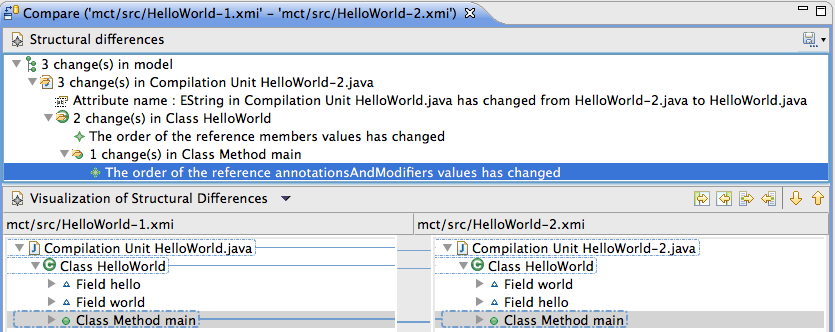
\includegraphics[width=\columnwidth]{code/emfcompare.png}
\caption{The differences found by EMFCompare on the two EMF models}\label{fig:1}
\end{figure}
Applying a structured diff algorithm~\footnote{EMFCompare, www.eclipse.org/emf/compare} to the EMF models corresponding to the abstract syntax structure of the two example Java programs\cite{DBLP:conf/sle/HeidenreichJSW09}), 3 changes are reported: one concerns the renamed compilation units, one concerns the class {\tt HelloWorld} for ``{\em the order of the reference members}'', and the final one concerns the method ``{\tt main}'' for ``{\em the order of reference annotationsAndModifiers values}''. 

In fact, none of the changes identified in this example is meaningful if the programmer only wants to see non-trivial
changes: just as adding a newline or some whitespaces would not change the syntax of the program, nor would swapping the keywords {\tt public} and {\tt static} in the declaration of the {\tt main} method make any semantic differences.

To find a meaningful change between two versions of a program, our proposed solution includes two major steps. \begin{itemize}\item {\em Step 1. Specification}: the programmer defines a number of annotations to the given grammar of the programs; \item {\em Step 2. Detection}: the tool generates two sets of transformations (normalisation, clone-removal) from the specification in Step 1 and applies these transformations to the two source programs to report the meaningful changes.\end{itemize} Figure~\ref{fig:overview} illustrates the workflow of a typical use case where the thin arrow indicates the manual specification step for the developer to annotate the given grammar; and the thick arrows indicate the automated transformation steps, for the mct system to generate the grammar refinement and transformation rules to detect meaningful changes from the programs in the CVS repository. 
\begin{figure}\centering
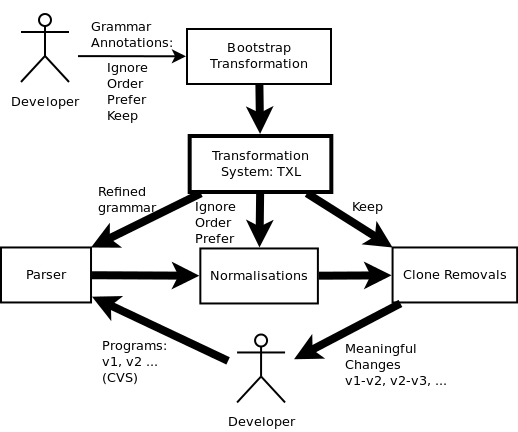
\includegraphics[width=\columnwidth]{code/overview}
\caption{Specifying and detecting meaningful changes, an overview}\label{fig:overview}
\end{figure}

\section{Specifying Relevant Changes}\label{sec:approach}

Before specifying our tool, we first define a few requirements for detecting {\em meaningful changes} through normalisation transformations.
\begin{definition}
{\bf Normalise into equivalence classes}.\label{defn:norm} A program $P$ is said to be {\em meaningfully equivalent} to program $P'$ if and only if $(P'=P) \vee (N(P') = N(P))$ where $N(P)$ is the normalisation transformation of $P$. In other words, $P'$ introduces no meaningful changes to $P$. Typically $N(P)$ is a many-to-one transformation.
\end{definition}

As discussed earlier, the exact meaning for `meaningful equivalent' in  the Definition~\ref{defn:norm} is intentionally left open for user to define by the normalisation function, because it depends on the purpose of the analysis and the relevance to the tasks. The definition provides the general criteria for determining whether a transformation is a suitable normalisation once it is clear what is meaningfully equivalent to the users: any trivial or irrelevant changes should be normalised to the same value. After the normalisation transformation is defined, the detection of the meaningful changes becomes comparing the two normalised programs. 

In principle, however, there can be infinite possible normalisations for defining an equivalent class. For example, adding any number of whitespaces can be regarded as normalisation transformations as opposed to removing the whitespaces. 
Therefore, such a normalisation transformation needs to be {\em terminable} by restricting the size of the targets.
\begin{definition}
{\bf Terminable normalisation.\label{defn:norm2}} A normalisation $N$ is {\em terminable} if $N(P)$ is smaller than $P$ in size.
\end{definition}
The {\em identity} transformation which preserves everything in the source is a normalisation, however it is trivial that all changes are meaningful if the identity is used as normalisation. According to Definition~\ref{defn:norm2}, we only consider the transformations that indeed make the output smaller than the input.

In the remainder of the paper, we focus on generating normalisation transformations based on elementary composable normalisations that can be derived from the language grammars. Since the language grammar is made of production rules,
one can start with the basic types of structural terms on each production rule, mandatory, optional, repeat and alternatives. For the optional/repeat terms, if one modifies it into the mandatory terms the transformation can violate the Definition~\ref{defn:norm2}. Similarly modifying optional to repeat could also introduce non-terminations. Therefore this leave us with three basic types of normalisations.
\begin{definition}
{\bf Elementary structural normalisations.\label{defn:norm3}} Let a production rule be $N \leftarrow (T_1? \ldots T_n*) [| \ldots] $ where $A$ is a non-terminal, and $T_i$ is the $i$-th term (which could be either terminal or non-terminal), and optionally the rule could contain more than one alternative sequence patterns. Every optional (denoted by `?') term can be {\em ignored} if with or without the value makes no difference to the developer; elements of the repeated (denoted by `*') term can be {\em ordered} if the ordering of the values are not important to the developer; and the whole element that matches with one mandatory alternative ( `$|$' )  can be {\em preferred} to a simpler values if a difference between the alternative rules are not significant to the developers.
\end{definition}

The three elementory structural normalisations preserve the validty of the normalised program in terms of the source programming language. %Based on the BNF, the production rules of programming languages are typically of three types,
%mandatory, optional, or repeat. 
\begin{property}
{\bf Composibility of syntax validty.\label{defn:norm4}} The normalised program by the three elementary transformations are valid programs in the {\em source} programming language.
\end{property}

The validity of the normalised programs is not a concern when the purpose of checking meaningful changes is not to obtain a compilable program. In such cases, one could choose to redefine the target grammar to be incompatible to the source language. On the other hand, if there is a simple alternative in the source language's production rule, such as semicolon, then it is useful to apply the Prefer rule to switch to a simpler alternative while preserving the source grammar in the transformed targets.

Also it is found that the elementary normalisations can be further customized. The unconditional ignored rule for an optional term `?' can be associated with a conditional check, for example in the API extraction example, one would remove the declaration if and only if it does not have a `public' or `protected' modifiers. Similarly, the ordered rule for repeating terms `*' can be customized to ascending or descending orders, and the ordering criteria can be associated with certain key' substructures.

The following property guarantees that a functional composition of the three basic normalisation transformations still satisfy the requirements of terminable normalisation.
\begin{property} {\bf Composibility of terminable normalisation}
If two basic normalisations $N_1$ and $N_2$ satisfy the terminable normalisation requirements in Definitions~\ref{defn:norm} and~\ref{defn:norm2}, then the functional composition $(N_1 \oplus N_2) (P) = N_2 (N_1(P))$ also satisfies the terminable normalisation requirements.
\end{property}

After each program revision is normalised, the next task is to detect the non-trivial changes. One extreme of  the methods is to apply an existing {\tt diff} algorithm, which in fact may or may not detect the exact differences.  Another extreme of the methods is to apply clone detection~\cite{DBLP:conf/iwpc/RoyC08a}. The benefit of applying clone detection is that one could take advantage of knowning the meaningful structures. Therefore, if the ordering is not imporant and as long as the normalised entities are the same, the clone detector could find them. On  the other hand, if the two entities are similar but not exactly the same, a meaningful context of the difference can be shown.
Not all language constructs should be considered as clones. E.g., the index variables of a for-loop are apparently not the best candidate to tell meaningful changes. It makes little sense to keep the for-loop structure while removing all the index variables.
To be able to specify which part of the language construct needs to be considered as clones to removal, another kind of annotation to the non-terminals are introduced as the following rule. 

\begin{definition}
{\bf Elementary structural clone removals.\label{defn:norm5}} Any entity in the grammar can be marked as possible clones such that a clone removal transformation can remove any duplicated occurrance. 
\end{definition}

In principle any parameterised AST-based clone detector could be used for this purpose. To illustrate in this paper we show the simpliest exact clones.

Table~\ref{table:rule} summarises the four elementary annotations to the meta-grammar for the normalisation/clone removals. Although they are by no means complete, we found that they are sufficient for many practical meaningful change detection tasks.
\begin{table*}\centering
\caption{Basic annotations to the terms in a TXL grammar}\label{table:rule}
\begin{tabular}{|c|c|c|c|}\hline
\bf Transformation & \bf Application scope & \bf TXL annotations & \bf Example \\\hline\hline
Ignore & Repeat/List ($*$), Optional ($|$) & [\ldots ignored when F] & [repeat member\_declaration \emph{ignored when Private}]\\\hline
Order & Repeat/List ($*$) & [\ldots ordered by F] & [member\_declaration \emph{ordered by Ascending}] \\\hline
Prefer & Alternative ($|$) & [\ldots preferred with C ] & [method\_body \emph{preferred with '; }] \\\hline
Keep & Any non-terminal term & [\ldots kept ] & [class\_body\_declaration \emph{kept}] \\\hline
\end{tabular}
\end{table*}

\subsection{A Running Example}\label{sec:example}
To illustrate the features of our method, here we use the example of the Java 5 grammar provided by the TXL site\footnote{http://txl.ca}, with 970 lines of code. Listing~\ref{listing:java0} selects a few production rules, with line numbers of the original Java5 grammar. In the conventions of TXL meta-grammar, a non-terminal is enbraced by square brackets, and a production rule is defined by the `define...end define' blocks. TXL is a functional programming language in which a transformation is defined by either a non-recursive {\tt function} or a recursive {\tt rule}~\cite{txl}.

\lstinputlisting[language=,identifierstyle=,caption={\tt cat -n java.grm},label=listing:java0]{code/java.rules0.grm}
\lstinputlisting[language=,identifierstyle=,numbers=left,numbersep=3pt,caption={\tt cat -n java.annotated.grm},label=listing:java1]{code/java.rules1.grm}

Lines 151-153 define a {\tt program} as a single instance of package declaration; Lines 158-162 define each package declaration to have an optional description of the package header, zero to many import declaration(s), before zero to many type declaration(s). Lines 197-201 define a type declaration as either one of three alternatives for, namely a class, an interface or an enum type. In these lines, [NL], [IN] or [EX] are predefined indentation tokens which will be ignored by the parser, but will be inserted by the unparser to pretty print the transformed code.  NL, IN or EX are respectively for new line, increasing and decreasing indention levels. Therefore the output has two lines per import declaration. 

Lines 377-379 define the method declaration as zero to many modifiers (as listed in Lines 254-267), plus an optional generic parameter, a type specifier, a method declarator, optional throws exception declarations and the method body. 
It is also notable that the method body is defined in Lines 407-410, which refers the block, defined in Lines 486-490, as a curly brace encloded array of zero to many declarations or statements.

It is possible to redefine the grammar of Java5 in TXL in many ways without necessarily changing the validity of a Java 5 program. For example, by replacing the two [NL] [NL] to a single [NL], one can already remove all the empty lines following the import statements. In the remainder of the section, we explain how normalisation is done by using these grammar rules as the input.

Comparing the annotated Java 5 grammar as shown in Listing~\ref{listing:java1} with the original in Listing~\ref{listing:java0}, it is clear that one only needs to ``redefine'' existing production rules while leaving other rules intact by simply including them (e.g., Line 1).

The redefined rules in Table~\ref{table:rule} are used or composed in some of the term extensions. Here we explain the rationale behind these extensions. First of all, the top level rule is modified from a singleton to one or optionally two instances of the programs (Lines 2-4). The reason for this is to allow the clone detection to work on the concatenated programs being compared to remove those inter-program clones such that the kept elements are all about different elements. The annotations ``\underbar{kept}'' are appended to the terms such as ``package\_header'' (Line 6), ``type\_declaration'' (Line 8), ``class\_body\_declaration'' (Line 12). These instruct a clone detector to compare these three types of entities for possible clones. Although the technique is similar, there is also a fundamental difference between general-purpose clone detection and cross-program clone-removal here. The purpose is not to show the clones, instead the opposite: those non-clones are the differences to be detected.
When a single program is provided as the source, of course, the transformations will then degenerate into just selecting the  parts of the program in which changes are embedded.

However, the ordering of elements or appearance of ignoreable details can get in the way of meaingful change detections. Therefore the normalisation transformations are required to be applied before the change detection step. 

Since one does not care whether a modifier is before another one or not (e.g., 'private static' is the same as 'static private'), the ordering of the elements in the array of {\tt repeat modifier}  (Line 378) is unimportant to the Java semantics. However, the default behaviour of TXL parser preserves the ordering of the modifiers in the parsing tree as they occur in the source program. To specify the ``Order'' normalisation, one only needs to insert the \underbar{ordered} at the end of the {\tt [repeat modifier]} term.

Furthermore, if one would like to normalise the elements by the descending order, a user-defined rule {\tt Descending} (Lines 29-34) can be added in Listing~\ref{listing:java1}. This is just to illustrate how easy it is to customize the comparison function, in case one would like to define a different key or ordering for the structure to be normalised. For the sake of identifying meaningful changes in this particular case, ordering the members ascendingly is the same as descendingly as long as the same criterion is applied to all source programs.

The Ignore annotation (\underbar{ignored}), on the other hand, will replace the optional or repeated terms by empty. The terms {\tt import\_declaration} at Line 7, {\tt class\_body\_declaration} at Line 12, are examples. In particular, the Ignore annotation to {\tt class\_body\_declaration} is conditional, it uses a user-defined function from Lines 23-28 to check when the term has not used the {\tt public} or {\tt protected} modifiers. As a result, it will achieve the effect of extracting API methods from all members. 

Without specifying such user-defined functions, the default behaviour of Ignore extension would simply ignore the term, just as what {\tt import\_declaration}. Because such terms are unconditionally ignored, therefore it is unnecessary to compose it with the Keep annotation as other sibling do. As a result, this will ignore the import statements in the API regardless, so any difference in such statements will not be considered as meaningful.

Finally, the Prefer annotation ({\underbar{preferred}) are appended to the terms that have more than one alternative expansions.
Our default implementation will transform any occurrence of other alternatives into the first one listed by the production rule.
For example, when the {\tt method\_body} at Line 16 is annotated by preferred, the production rule from Lines 18-21 are used to transform any block into a semicolon because it is the preferred alternative. Note that for this to work, users need to modify
the production rule of {\tt method\_body} in the original grammar Lines 407-410 to swap the two alternatives, which is perfectly doable without modifying the semantics of the Java5 grammar.

\subsection{Brief discussion about the implementation}
The meaningful change detection tool {\tt mct} is implemented completely as a TXL program. The first part of the implementation is an extension to the TXL's metagrammar {\tt txl.grm}. Listing~\ref{listing:extend} shows the extension to the existing {\tt typeSpec} rule and the addition of four annotation rules {\tt orderedBy}, {\tt ignoredWhen}, {\tt preferred} and {\tt kept}.
\lstinputlisting[language=,identifierstyle=,numbers=left,numbersep=2pt,caption={\tt cat -n norm.grm},label=listing:extend]{code/norm.grm}
 
The second part of the implementation is a specification of the normalisation transformations. Limited by space, here we only show a simplified Listing~\ref{listing:normalise} for the Order extension. It generates rules for eliminating {\tt ordered} annotations for the generated grammar to be recognizable by TXL at runtime, and for producing rules for ordering the
terms parsed as {\tt [repeat X]}. 

A TXL program can be understood top-down from the back. Lines 44-64 specify how to generate the transformation rules {\tt Rules} on the fly by checking every {\tt redefineStatement} in the TXL grammar such as those in Listings~\ref{listing:java1}.  For each occurrence of {\tt [repeat X ordered by F]}, the transformation in Lines 9-31 is invoked to generate a rule such as those instantiated in Lines 22-27. These rules have unique names constructed from the names of the {\tt redefineStatement} and the term {\tt X}. By the end of the main transformation, the rule in Lines 2-8 are applied to eliminate the Order annotations from the extended grammar.
\lstinputlisting[language=,identifierstyle=,numbers=left,numbersep=2pt,caption={\tt cat -n norm.Txl},label=listing:normalise]{code/norm.Txl}
\subsection{Generated normalisation transformation}
The above generic implementation is done on the meta-grammar of TXL. When it is applied to a concrete TXL grammar, such as the one specified in Listing~\ref{listing:java1}, a concrete normalisation transformation is produced in the original syntax of TXL, as shown in Listing~\ref{listing:output}. Lines 1-9 are the same as the original rules in the Listing~\ref{listing:java0} because of the elimination rule. Lines 10-17 are generated from the {\tt [repeat method\_declaration]} of the {\tt orderedBy} annotations from Listing~\ref{listing:java1}, using the user-defined comparison function {\tt Descending}, which was listed in Lines 29-34 in Listing~\ref{listing:java1}. 
\lstinputlisting[language=,identifierstyle=,numbers=left,caption={\tt cat -n java.Txl},label=listing:output]{code/java.Txl}

In brief, the above extension of Java5 grammar has 8 annotations added by the user, plus 1 user-defined string comparison rule for sorting the nodes in inverse alphabatical order and 1 user-defined function for selecting non-API members to be removed.
\subsection{The normalised programs and relevant changes}
We have implemented the processor of all the four types of elementary annotations using TXL, which generates all transformation rules per annotated term. Applying the composed {\tt mct}  transformation to the two Java programs in Listings~\ref{listing:1} and~\ref{listing:2}, separately, the same result is obtained, as shown in in Listing~\ref{listing:result5}. Both {\tt hello} and {\tt world} members are removed because they are not public nor protected members of the class. The {\tt main} method has the modifiers ordered ascendingly as {\tt public static}, whilst its method body is replaced by the preferred simplification semicolon alternative. 

When the same transformation is applied to the concatenated inputs of both programs, the clone removal step runs to correctly remove all the clones according to the terms annotated by ``kept''. As a result, their is no longer anything left after the clone removal, leaving the output empty as shown in Listing~\ref{listing:result4}.
\lstinputlisting[numbers=left,caption={\tt mct HelloWorld.java},label=listing:result5]{code/HelloWorld-2.norm}
\lstinputlisting[numbers=left,caption={\tt cat HelloWorld.java HelloWorld-2.java > HelloWorld-2.pair \\ mct HelloWorld-2.pair java.Txl},label=listing:result4]{code/HelloWorld-2.mct}

\section{Performance evaluation}\label{sec:experiment}
To evaluate the {\tt mct} tool, we experimented on three evolving programs, namely {\tt gmf}, {\tt jhotdraw} in Java and {\tt Uart16650} in Verilog. These benchmark programs are in the public domain: {\tt JHotDraw} is a  GUI framework for technical and structured Graphics, which was studied for the API evolution and refactoring opportunities~\cite{DBLP:journals/smr/DigJ06}; {\tt GMF} is a model-driven code generator for Eclipse Graph Editors, which was  studied for the evolution of the model/code co-evolution~\cite{DBLP:conf/sle/HerrmannsdoerferRW09}; {\tt OpenCores Uart16650} is a specification of FIFO queue for hardware, which was used for the study of Verilog Diff~\cite{Duley:2010:PDA:1858996.1859093}.

To apply to these programs, we first defined the relevant changes based on their corresponding programming languages. Table~\ref{table:2} lists the size of the meta-grammar (txl.grm), Java 5 grammar (java5.Txl) and the Verilog grammars (v.Txl). The {\tt mct} tool is implemented as {\tt mct.Txl} as 19 rules that transform the 7 extended terms. The Java API normalisation tool is implemented by redefining 21 terms using 7 Keep, 17 Order, 1 Ignore and 2 Prefer annotations, and 2 user-defined rules; as a result, 47 new transformation rules are generated. The Verilog annotations include 4 Keep and 5 Order, which generates 12 transformation rules. 

\begin{table}\centering
\caption{Size of the fully extended grammars\label{table:2}}
\begin{tabular}{| r || r | r | r | r |  r |  r |  r  |}\hline
{\bf Grammar} & description & LOC & Terms &  Rules \\  \hline\hline
txl.grm & TXL meta-grammar & 408 & 58 & 0 \\
mct.Txl & Implementation & 544 & 7 & 20 \\ \hline
java5.Txl & Java 5 grammar &  976 & 168 & 0 \\
java.norm & annotation & 123 & 21 & 2 \\ 
java.Txl & result & 721  & 27 & 49  \\\hline  
v.Txl & Verilog grammar & 233 &  37 &  1\\
v.norm & annotation & 45 &  9 & 0 \\
verilog.Txl & result & 191 &  11 & 12 \\\hline
%problem.grm &  problem frames & 82 & 5 \\ \hline
%json.grm & JSON format for Javascript & 36 & \\ \hline
%yaml.grm & YAML serialisation format & 94 & \\ \hline
%uncal.grm & UNQL+ format & 111  & \\\hline
%q7.grm & i* requirements &  100 & \\\hline
%argument.grm & Argumentation & 41 & \\\hline
%dot.grm & Graphviz directed graph & 79 & \\\hline
%ec.grm & Event calculus &  41 & \\\hline
\hline\end{tabular}
\end{table}


Then we accessed the history of {\tt gmf} and {\tt jhotdraw} by analysing all commits from their public CVS repositories; whilst we were using the same set of selected revisions of {\tt Uart16650} provided by Dulay et al~\cite{Duley:2010:PDA:1858996.1859093}.
Table~\ref{table:3} lists the size metrics of the example programs. The `File' column shows the number of files stored in the repository, while the `Rev.' columns shows the number of revisions of these files. The `LOC' column indicates the lines of code of all the revisions, the `LOC$_m$' columns shows the lines of code after the normalisation transformations. The `Change column shows the number of changes detected by the {\tt diff} utility, and `Change$_m$' shows the number of changes detected by the {\tt mct} tool. 
\begin{table*}\centering
\caption{Size of the programs\label{table:3}}
\begin{tabular}{| r || r | r || r | r |r | r || r| r|  r | r |}\hline
{\bf Program} & File & Rev. & LOC & LOC$_d$ & LOC$_l$ & LOC$_{m1}$ & LOC$_{m2}$ &Change  & Change$_m$  \\  \hline\hline
{\tt jhotdraw} & 1,297 & & & & &\\\hline
{\tt gmf} & 8,809 &  & &  & & \\\hline
{\tt uart16650} & 12 & 128 & 51,551 & 28,805 & & \\\hline
\hline\end{tabular}
\end{table*}

%
%%\subsection{Efficiency: The evolution of JHotDraw code}
%Every single revision of every RCS file with the extension of {\tt ,v}. Then we compare every consequent files by the {\tt diff}, {\tt ldiff} and {\tt mct} commands. If the differences are non-empty, we count the number of revisions,  number of non-empty differences and the time it took to compute the results.
%\begin{table}\centering
%\caption{Performance of change detction\label{table:2}}
%\begin{tabular}{| r || r | r | r | r ||}\hline
%{\bf GMF} &  {\bf cmts} & {\bf Rev.} & {\bf Hunks} & {\bf Time} \\\hline\hline
%{\tt diff} & with & 17,521 & 93,254 & \\\hline
%{\tt   + diff} & w/o & 15,116 & 41,212 & \\\hline
%{\tt ldiff} & with &  & & \\\hline
%{\tt txl + ldiff} & w/o  &  & & \\\hline
%{\tt mct + diff} &w/o  & & & \\\hline
%{\tt mct + ldiff} &w/o  & & & \\\hline
%\hline\end{tabular}
%\end{table}

\section{Related work}\label{sec:related}
\subsection{Grammarware}
 
~\cite{klint05tosem}
   
\subsection{Transformation systems}

   `TXL` [cordy02]
   
\subsection{Model Diff}
Xing and Stroulia~\cite{xing05ase} propose an approach to recover UML models from java code, and compares them producing a tree of structural changes, which reports the differences between the
two design versions.  Their approach is specific to UML. It uses similarity metrics for names and structures in order to determine various changes made to them. (This paper discusses various types of change operations, the correctness of their tool for those operations. So we can follow their example)

Apiwattanapong et al~\cite{Apiwattanapong:2004:DAO:1025115.1025202} present a graph-based algorithm for differencing object-orienetd programs. Since their approach and the tool JDiff is geared towards Java, there is explicit support Java-specific features, such as the exception hierarchy.



% Schmidt and Gloetzner~\cite{schmidt08icse} describe an approach that integrates the SiDiff 

There are several differencing tool working at the semantic level. Jackson and Ladd~\cite{Jackson:1994:SDT:645543.655704} uses dependency between input and output variables of a procedure as a way to dectect certain changes. The depenedncy is represented as a graph and any difference in two graphs is taken as a change to the semantics of the procedure. There are, of course, changes that affect the semantics but not the dependency graph, such as the changes in constants.

Kawaguchi et al~\cite{Kawaguchietal2010} a static semantic diff tool called SymDiff, which uses the notion of partial/conditional equivalence where two versions of a program is equivalent for a subset of inputs.  The tool can infer certain conditions of equivalence, and therefore behavioural differences can be lazily computed. 

Brunet et at~\cite{brunet06gamma} defines some chanllenges in model mangements including the operations merge, match, diff, split and slice, as well as the properties that need to be preserved by these operations. These operations and properties are independent of models and modelling languages.

Duley et al~\cite{Duley:2010:PDA:1858996.1859093} present VDiff for differencing non-sequential, ``position independent'' Verilog programs. Their algorithm first extracts the abstract syntax trees of the programs, and match the subtrees in the ASTs whilst traversing them top-down. Furthermore, Boolean expressions are checked using a SAT solver and the results of differencing are presented as Verilog-specific change types.

Loh and Kim~\cite{Loh:2010:LPD:1810295.1810348,Kim:2009:DRS:1555001.1555046} present the LSDiff tool which automatically identifies structural changes as logic rules.

\section{Conclusions and future work}\label{sec:conclude}

   Scalability
   
   Meta-changes: Changes to the Transformations
   
   We believe there is no need for infinite meta-levels. One example is `KM3` or `MOF`, although in principle there is always a possibility to ask for meta-level 
   changes, typically the language is less likely to change than the program.
   
   How to make use of `iChange` for runtime adaptation?
   
   The deployed system also need to adapt dynamically to the changes in its environment at runtime.
\cite{klint05tosem}  
\cite{cordy02} 
\cite{txl} 
\cite{wenzel08icse} 
\cite{xing05ase} 
\cite{fluri07tse}
\cite{schmidt08icse} 
\cite{wenzel08icsm}
\cite{brunet06gamma}
\cite{degenais08icse}
\cite{canfora09software}
%\bibliographystyle{plain}
%\balancecolumns
\begin{small}
\balance
\bibliographystyle{IEEEtran}
\bibliography{meaningful}
\end{small}
\end{document}

%Similarly, graphs used in requirements/design modeling activities typically allow moving nodes around in order to present the model in a different physical layout, whilst the topology is preserved. Often such layout changes are saved through the serialisation, leading to false alerts that the software design has changed. 
%These are just a few examples of how important and challenging it is to detect meaningful changes. The general problem remains the same. 

%{\em customized} to detect different kinds of changes, e.g., {\tt diff} either accepts or rejects whitespace differences depending on whether or not a command line switch {\tt -w} has been used. Such choices, however, can be misused easily by programmers who, for example, accept whitespaces changes in Python programs, or reject those in Java programs. Specific to the needs of programmers, it is often the case that whitespaces within one region of the program require attention while those within another are irrelevant. A global choice made for the {\tt diff}   is inappropriate in such cases. 

%
%materialised views to various artifacts including requirements models, UML diagrams and programming languages. Such specific views are defined declaratively as a lightweight extension to the grammar of the subject languages. 

%A program is considered meaningfully different from another only when it has non-trivial changes; otherwise it is considered meaningfully the same even after introducing trivial changes by, e.g., adding or deleting whitespaces, or by reordering the type modifiers in method declarations, etc. 
%\subsection{Programs and {\tt diff / ldiff}}
%
%\subsection{Graphs and serialisation/abstraction}
%Graph models have similar problems, if not worse. To illustrate this point, consider the two simple diagrams drawn by an Eclipse-based graphical modeling tool in Figure~\ref{fig:1}\footnote{Most UML modeling tools based on Eclipse also use the same underlying model-driven technology to create the editor plugins for editing and saving EMF/GMF models such as class diagrams.}.
%Although the diagram below has changed the diagram above it by placing the ellipse node (Requirement) on the left rather than on the right, and by filling different colors into the shapes, the topology of the graph and the content of the corresponding EMF model remain the same, according to the domain-specific language defined in Problem Frames~\cite{jackson01}.
%\begin{figure}
%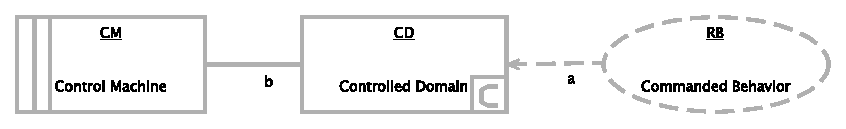
\includegraphics[width=\columnwidth]{code/CommandedBehaviour1}
%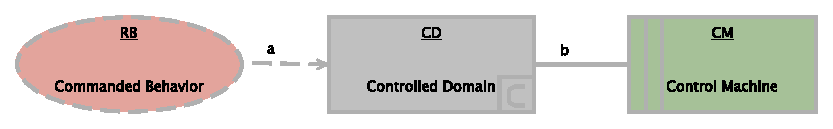
\includegraphics[width=\columnwidth]{code/CommandedBehaviour2}
%\caption{Equivalent problem frame diagrams: commanded behaviour}\label{fig:1}
%\end{figure}
%
%The underlying {\tt HashMap} in the modeling tool, however, could serialise the modeling elements by different (and rather random) orderings, making it more difficult for a simple diff tool to detect meaningful changes to their EMF models. The EMF model can be saved as an equivalent model in corresponding domain-specific (textual modeling) language (DSL) such as those specified using the Eclipse Xtext framework~\footnote{http://eclipse.org/xtext} (e.g., List~\ref{listing:xtext}). 
% \lstinputlisting[language=,identifierstyle=,numbers=left,emph={problem,event},stringstyle=\color{red},caption={\tt cat -n CommandedBehaviour.problem},label=listing:xtext] {code/CommandedBehaviour1.problem}
%Besides the whitespace problems, in this example, the phenomena are not alphabetically ordered, nor do the domain nodes. 
%One can imagine easily that swapping two nodes or two phenomena in this serialised model could lead to false alarms which in fact do not require attention by the designers. Comparing two models at the EMF level using a tool such as {\tt EMFcompare}~\footnote{http://eclipse.org/emfcompare}, one could avoid such false alarms\footnote{TO CHECK}.
%
%Moreover, analysts/designers do not always want to view every detail of the modeling elements. For example, the phenomena of the domain nodes in a problem diagram, or the exact declaration of the class methods in a class diagram, are not viewed when the analyst/designers is concentrating on the structural relationship between the larger entities (domain interfaces or class hiearchies). As such, an abstraction transformation is often required before one compare meaningful structures rather than the meaningless details that should be hidden from the view. Of course, programmers may sometimes want to compare the details of the exact declarations of method, while still would wish to ignore the detail implementation of the method bodies. Therefore for the same model (e.g., graph) it is helpful to allow an abstraction as the preprocessing step for a meaningful comparison.
%
%Although not mandatory, for pragmatic reasons it is preferable to have the outputs of normalisation readily compared by reusing line-based diff tools. 
%\begin{definition}
%{\bf Diff-friendly Normalisation.\label{defn:norm3}} A normalisation $N$ is diff-friendly, if any line in the normalised program $N(P)$ has at most one meaningful changes.
%\end{definition}


%Given that a program is expressed in programming languages consist of production rules~\cite{Aho:1986:CPT:6448}, our normalisation tool {\tt mct} needs to satisfy the following requirements, in order to handle those examples motivated in the previous section:
%\begin{enumerate}
%\item [R1] Ignore the trivial differences in optional or repetitive {\em terminals} in the production rules;
%\item [R2] Ignore certain non-terminals in the rules according to the needs of further abstraction;
%\item [R3] Ignore the ordering of the unordered collections by ordering them sequentially, such that two collections of the same set of elements are the same sequences;
%\item [R4] Carry out the normalisation transformations on the fly, without any user intervention once the grammar rules are extended using the annotations for [R1], [R2] and [R3].
%\item [R5] (optional) Occupy at east one line per non-terminal;
%\item [R6] (optional) Make sure the normalised program is still a valid program in the original grammar.
%\end{enumerate}


%The requirement [R1] is sufficient to ignore all unnecessary non-terminals in the output program. Such normalisations help focus the comparison more on the abstract syntax rather than on the concrete syntax, because it is the abstract syntax that carries the meaning of the representation while the concrete syntax (reflected by the non-terminals) are merely the auxiliary tokens to parse. The default {\em unparse} functionality of TXL~\cite{txl} can already satisfy the requirement of removing extra whitespaces. To remove the extra non-terminals, we must introduce the ``ignore'' attribute to the type specification, such as {\tt [opt 'terminal \underbar{'ignore}] }. Requirement [R2] is similar to that of [R1], but now it is the non-terminals that are to be ignored for the abstraction purpose. 
%
%Requirement [R3] is useful especially when users knows when a list or an array of literals (tokens and non-terminals) is in fact unordered (e.g., the type modifiers in Java, the phenomena in problem frames), therefore combinatory numbers of possible differences can be removed by ordering the elements in the same way. By default, we can use the serialised string of the literal and sort them in ascending ordering. Of course, such ordering can be made more flexible by allowing users to specify the appropriate ordering key/transformations. Examples of this extension are {\tt [ repeat X \underbar{ordered} ] } where the non-terminal X will be ordered in the normalised program; or {\tt [list X \underbar{ordered by Y}] } where the non-terminal X will be ordered by the comparison rule specified by {\tt Y(X)}. In other words, users can choose to order the elements in descending order, or by the ordering of a particular key field. 
%
%Satisfying the requirement [R4] would allow the transformation from the program to a `simplified' grammar to be generated on the fly, appending additional transformation rules by either ignoring or ordering the literals that have been extended.  The implementation of [R4] is done through the technique of {\em bootstrapping}, that is, to reflectively annotate certain literals in the TXL meta-grammar using the {\tt ignore} and {\tt ordered by} extensions given that the TXL grammar itself is expressed in TXL as a meta-grammar. By processing each annotation in the context of the production rules, it produces a context-aware rule for the transformation on-the-fly. Then the annotations are stripped off by default, which produces a pure-TXL grammar without the annotations, while additional rules based on those removed annotations are combined together. This combined grammar specification is then used to parse the programs in the original language and produces the normalised programs. 
%
%Optionally, requirement [R5] can be  enforced by inserting a new line directive  {\tt \underbar {[NL]}} to the end of each non-terminal literal in the production rules. Sometimes the normalised program does not have to be a valid program in the same grammar because removing the details may make the output no longer a valid program, therefore [R6] is the default preference applied if the user would like to preserve the program syntax as well. For example, the abstracted program is still in valid Java syntax by retaining the \{ \} braces while hiding the body of a Java method.

%\lstinputlisting[language=,identifierstyle=,numbers=left,caption={\tt cat -n problem.rules2.grammar},label=listing:problem2]{code/problem.rules2.grm}
%Of course, the user may choose to ignore certain information to further abstract the normalised structure, e.g., as indicated in Listing~\ref{listing:problem3}, the {\tt details} can be ignored by using {\tt ignore} at the end of the optional part {\tt [opt details]}. 
%\lstinputlisting[language=,identifierstyle=,numbers=left,caption={\tt cat -n problem.rules3.grammar},label=listing:problem3]{code/problem.rules3.grm}
%Note that using the above extensions after {\tt opt}, {\tt repeat} and {\tt list} parts, the normalised programs will still be valid for the original syntax.

%From Listing~\ref{listing:xtext}, applying the transformation in Listing~\ref{listing:output}, the normalised program is shown in Listing~\ref{listing:result} where the elements are descending alphabetically, while the phenomena are ascending alphabetically.
%\lstinputlisting[language=,identifierstyle=,numbers=left,caption={\tt cat -n CommandedBehaviour.n1.problem},label=listing:result]{code/CommandedBehaviour.normalised.problem}
%Alternatively when the {\tt [opt details ignored]} is specified, Listing~\ref{listing:result2} shows the resulting abstraction where the details are ommitted.
%\lstinputlisting[language=,identifierstyle=,numbers=left,caption={\tt cat -n CommandedBehaviour.n2.problem},label=listing:result2]{code/CommandedBehaviour2.normalised.problem}
%As long as the same normalisation is used, two programs with meaningfully changes will be detected while the opposite will not.
